\documentclass[a4paper,10pt]{report}
\usepackage[utf8]{inputenc}
\usepackage[pdftex]{graphicx}
\usepackage{fancyvrb}
\usepackage{hyperref}
\usepackage{helvet}
\usepackage{amsmath}


%opening
\title{Sistema de transmisión segura punto a punto y multipunto en medios compartidos.}
\author{Alfredo Ortega}
\makeindex

\begin{document}

\maketitle
\newpage
\tableofcontents
\newpage
%\begin{abstract}
%Sistema de transmisión segura punto a punto y multipunto en medios compartidos.
%\end{abstract}

\section{Introducción}
En este trabajo se presenta una tecnica novedosa de transmisión de datos en redes de tipo broadcast de manera criptograficamente segura utilizando tecnicas de espectro expandido.



\section{Estado del arte}
Los sistemas de comunicaciones opticos han echo posible las comunicaciones modernas, tecnologias como Internet comunicaciones celulares no son posibles sin una infraestructura optica de comunicaciones de alta velocidad.
Generalmente las redes de alta velocidad son switcheadas y sobre la capa fisica solo recientemente han sido utilizadas modulaciones y codificaciones mas complejas que un simple Xon-Xoff.
El Backbone ha evolucionado recientemente de 10Gbps, a 40 y 100Gbps, en donde se comienzan utilizan modulaciones de tipo WDM y modulacion en fase. Estas redes son generalmente switcheadas, no del tipo broadcast.
Existen redes de tipo broadcast donde existen ventajas como un sistema de ruteo mucho mas simple que puede ser totalmente optico, pero varios problemas como tener que compartir el ancho de banda, y problemas de seguridad inherentes al enviar la informacion a todos los nodos de la red. Este trabajo apunta a solucionar este ultimo problema.

\subsection{Códigos correctores de errores}
\subsubsection{Viterbi/Convolucional}

\subsection{Espectro ensanchado}
\label{espectroensanchado}
El espectro ensanchado, Spread Spectrum o CDMA es una tecnica donde se utiliza mucho mas espectro del medio de transmisión que el necesario para la transmisión correcta de los datos.
Los origines datan del 1900, cuando Nicola Tesla patentó el concepto de \textit{"Frequency hopping"}.
El spreading de la señal tiene varias ventajas:
\begin{enumerate} 
\item Resistencia al espionaje, ya que solamente las partes que conocen la señal de spreading pueden decodificar la señal original
\item Resistencia contra interferencias de banda angosta (No a interferencias de banda ancha como el ruido térmico)
\item Capacidad de acceso múltiple. Varios usuario pueden transmitir en la misma frecuencia mientras utilicen diferentes códigos.
\end{enumerate} 
Adicionalmente, al guiarse la señal expandida con un generador pseudo-aleatorio o PRBS, se puede agregar privacidad a la comunicación haciendo imposible decodificar los datos sin tener los parámetros del PRBS.

A su vez, se puede expandir la señal en tres dominios:
\begin{enumerate} 
\item Direct Sequence (CDMA): Se expande la señal multiplicándola (XOR) con la señal de spreading, generalmente mucho más rápida. Este método es el utilizado en WiFi y WiMAX, redes 3G de celulares, etc.
\item Frecuency Hopping: La señal de spreading es utilizada para variar la frecuencia portadora de la señal original. Este método es utilizado por ejemplo en BlueTooth. (Se utiliza Adaptive Frequency Hopping, un método para evitar frecuencias con mucha interferencia)
\item Time Hopping: La señal de datos no transmite todo el tiempo, sino que sufre de un delay que depende de la señal de spreading. Este método no es muy utilizado aunque lo estudiaremos detenidamente en nuestro caso ya que es muy sencillo de implementar con los recursos de los que disponemos.
\end{enumerate} 


La desventaja del expectro expandido, que es utilizar mucho espectro por bits transmitido, o lo que tambien se denomina baja densidad espectral, a veces no afecta demasiado al tener el canal una cantidad disponible de espectro mucho mayor a la utilizada. Un ejemplo de un protocolo de comunicaciones que utiliza CDMA es el protocolo WIFI, en todas sus versiones.

\subsection{Códigos de generación pseudo-aleatorio}
Para que un codigo CDMA pueda utilizarse para obtener privacidad en la comunicacion, es necesario que el parametro a expandir, sea la frecuencia, el tiempo o el codigo utilizado, sea guiado o seleccionado por un generado pseudo-aleatorio o PRBS, que son algoritmos que basados en un parametro de inicializacion o semilla, son capaces de generar un stream de numeros aparentemente aleatorios, pero en realidad totalmente deterministicos. 
Es necesario que los nodos que participen de la comunicacion puedan generar exactamente la misma secuencia y compartan el parametro de generacion o semilla. Esto es equivalente a lo que en criptografia se denomina un algoritmo criptografico simétrico.
Existen muchas maneras y algoritmos de generar streams pseudo-aleatorios. Algunos algoritmos estan optimizados para que su periodo (la cantidad de numeros en su salida antes que el patron se repita) sea enorme, como por ejemplo el algoritmo Mersenne-twister.
Otro parametro deseable en un PRBS es su sencillez y rapidez. Un generadores PRBS muy popular se denomina Lineal Congruential Generator y solo precisa de dos operaciones, una multiplicacion y una suma.

Estos ejemplos carecen de una caracteristica fundamental requerida en nuestro sistema: Que no se puedan predecir. Esta simple caracteristica no es en realidad trivial ya que muchas tecnicas existen para inferir datos acerca del generador PRBS, lo que supondria una falla en la seguridad de un sistema basado en dicho generador. Para evitar estos problemas existen los llamados generadores PRBS criptograficamente seguros. Como ejemplo podemos nombrar a los generadores shrinking o self-shrinking.

\subsection{Seguridad}
La propuesta es utilizar un sistema de espectro expandido con el objetivo principal de lograr la privacidad del canal al nivel fisico.
Se fijaron los siguientes parametros de seguridad:

. El sistema debe proveer confidencialidad, integridad y autenticidad de los datos.
. El sistema debe ser seguro sin importar la cantidad de clientes existentes o los datos que transmiten
. Un atacante no debe poder identificar los datos de un cliente, aunque controle todos los demas nodos de la red.

Con estos parametros se busco el algoritmo CDMA adecuado. Las caracteristicas de un sistema optico hacen muy complejo el hardware requerido para lograr CDMA o Frequency-Hopping, pero implementar Time-hopping no presenta costo ni dificultad adicional, asi que este fue el seleccionado para la implementacion de seguridad.
Varios algoritmos de asignacion del time-slot fueron analizados. Se necesita que la salida de los mismos sean códigos ortogonales, o sea, deben poseer un generador capaz de crear streams pseudo-aleatorios que nunca coincidan para no generar colisiones entre los clientes. Esto no es trivial sin compartir algun tipo de información entre todos los clientes, lo que debilita la seguridad del sistema. Por ejemplo, codigos existentes llamados gold-codes permiten la generacion de multiples secuencias con baja cross-correlacion, muy util para coordinar dispositivos que comparten el medio. Pero desde el punto de vista de la seguridad, este codigo es trivialmente derrotado. Por ejemplo en un esquema donde un atacante controla todos los canales menos uno, el atacante podria simplemente dejar de transmitir y revelar la secuencia utilizada por la victima, que forzosamente estara utilizando el canal restante.

Se decidio por utilizar una codificacion trivial: Seleccionar el time-slot de acuerdo a una secuencia criptograficamente segura estandard, totalmente independiente de los otros nodos. Es demostrable que esta decision produce un sistema extremadamente simple y seguro. Como contrapartido, produce una cantidad muy elevada de colisiones que aumenta exponencialmente con el numero de clientes. Sin embargo, estas colisiones pueden ser corregidas mediante codificacion adicional, y se logro una utilizacion de canal muy cercana al maximo teorico como se demostrara en la proxima seccion. De echo, es en esta codificacion adicional donde reside el principal aporte de esta tesis.

\subsubsection{Security considerations and cypher strength}\label{security}
%% extraido de dline-pub.tex
There are several aspects of security to a communication channel: Authentication, reliability, confidentiality, and integrity.
The scheme presented in this paper uses CDMA to provide confidentiality, reliability, and integrity between two or more parties, and is equivalent to a shared-key symmetric encryption scheme where the shared key is used to initialise the PRNG.
Additional aspects like authentication can be implemented using logical-layer protocols.
We specifically designed the proposed system taking into consideration attacks of the sort presented in Ref. \cite{Shake:05}.

As system security relies on the strength of its PRNG, special care must be observed in the selection and implementation of a suitable cryptographically strong algorithm.
The proposed PRBS is non-linear, e.g., as in a self-shrinking generator~\cite{Meier:94}.
Additionally the user's key is never broadcast to the network, so key distribution must be performed beforehand using a secure channel.

We address an additional vulnerability inherent to optical systems arranged as a star network: CDMA algorithms depend on interference for confidentiality.
However, in an optical star-topology there are locations where little or no interference among users is present, for instance, next to the transmitter output of an end user the signal power is high and can be singled out from the background noise.
Note that even if the hypothetical eavesdropper can locate and observe the bits of the transmitted symbol, they cannot infer any information.
As positions within the data frame can overlap, the eavesdropper will observe a symbol with a HW between 1 and HW$\times$K, but it is not possible to reconstruct the right order of the bits without the PRNG seed.

Most encryption algorithms rely on XORing (the case of the RC4 encryption algorithm), a combination of substituting/scrambling of the bits before transmission (AES and DES encryption algorithms), or more complex transformations (RSA or Elliptic Curve algorithms), see Ref.~\cite{Menezes:1996:HAC:548089}.
However, these techniques necessarily modify the Hamming weight of every symbol in a way that is not optimal for our CDMA scheme as it increases intersymbol interference.
As the presented algorithm relies on time-hopping CDMA, it effectively encrypts symbols while maintaining the desirable low Hamming weight, increasing total bandwidth utilisation as shown in Fig.~\ref{fig_use}.

\begin{figure}[t]
  \centering
  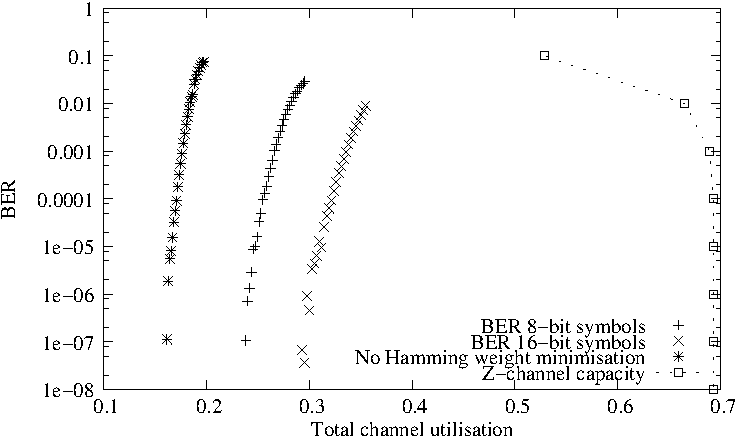
\includegraphics[width=0.48 \textwidth]{BERvsChannel} 
  \caption{Utilisation of the 10 Gbps channel. Each one of the 123 to 158 users transmitted 1 Gbit of data. Note the improvement in bandwidth utilisation compared to that in~\cite{ortega11}.}
  \label{fig_use}
\end{figure}

In contrast to TDMA, in our scheme the eavesdropper needs to intercept every optical fibre to reliably identify each end user as they are anonymised after passing through the central hub.



\section{Sistema propuesto (teoría y simulaciones)}

Se propone un sistema de comunicaciones óptico con una estructura de hub como se aprecia en la figura \ref{fig_hub}. Utilizando este Diseño físico con una etapa adicional de codificación y correccion de errores. El hub central es una etapa totalmente óptica que puede o no estar amplificada. Con la amplificacion optica se incrementa notablemente el rango, de 5 km a mas de 20 km.
La pila de codificación se detalla en la figura \ref{fig_stack} donde puede verse un arreglo convencional, excepto en la ultima 

\begin{figure}[t]
\centering
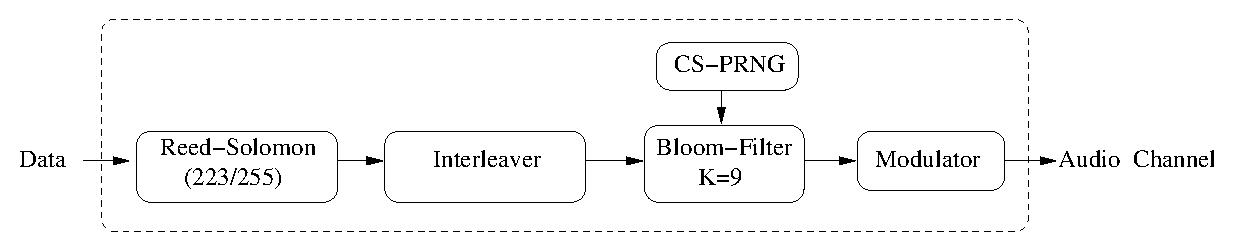
\includegraphics[width=0.9 \textwidth]{Soft-stack2.eps} 
\caption{Etapas del sistema de comunicaciones}
\label{fig_comstack}
\end{figure}

\subsection{Códigos correctores de errores}

Todo sistema de comunicaciones posee errores que deben ser corregidos antes que los datos sean procesados. Una técnica muy utilizada es la de utilizar un algoritmo de detección y retransmisión.
La idea de un código corrector de errores esta relacionada con la técnica de espectro expandido, siendo ambas métodos que ayudan a la transmisión de la información reduciendo la entropía de la información transmitida, o lo que es lo mismo, aumentando la redundancia de la información. En particular, los sistemas de comunicaciones modernos hacen uso de los métodos de Forward Error Correction (FEC) que no necesitan de retransmisiones.



\subsubsection{Reed-Solomon}
Se utilizo un codigo de Reed-Solomon standard 223/255, esto significa que se tienen 32 bytes de paridad por cada 223 bytes de datos, y se pueden corregir hasta 16 bytes. Se utilizo la librería de Phil Karn, y no se utilizaron los bits de sindrome para mejorar la correccion. Todo error conocido es descartado.
Con posibilidad de error de simbolo P, la posibilidad de error de un codigo reed-solomon R(n/k) es:
$$P_{rs}= \sum_{k=(\frac{n-k}{2}+1)}^{n} \binom{L}{i} * P^{i} * (1-P)^{L-i} $$

\subsubsection{LDPC}
El esquema de corrección de errores LDPC (Low Density Parity Check) es muy utilizado actualmente debido a su gran capacidad de corrección de errores, en algunos casos muy cercana a la máxima capacidad teórica del canal.
Antes de ahondar en la descripción de este algoritmo cabe aclarar que a pesar de ser utilizado para ciertos modelos durante la primera fase de la investigación, fue descartado en la versión final por un modelo mas simple y con menos requerimientos de hardware que presenta una performance similar desde el punto de vista de corrección de errores.
Básicamente es un código lineal que utiliza una matriz de paridad grande y dispersa.
La matriz H es tal que cualquier codeword valido x cumple con $H*x=0$

\paragraph{LDPC: Generador de matriz}
La matriz generadora puede crearse facilmente si H es de la forma $[D|I]$, simplemente formando la matriz:
$$G=[I|D']$$
Donde D' es la transpuesta de la matriz D
Para la generacion de la matriz se opto por utilizar un algoritmo random y luego aplicando algunos tests, para lograr una matriz sistemática de rate entero (1/2, 1/3, etc.)
Para verificar se G genera vectores cuya matriz de paridad es H, puede verificarse que:
$$ H*G'=0 $$

Podemos definir la matriz de paridad H como una matriz de paridad que tenga mas de 3 unos por fila y una cantidad similar por columna. Buenos resultados se obtienen a partir de matrices de 200x100.
Se puede comenzar por una matriz vacía $H = 0$ del tamaño deseado, y ir agregándole unos al azar. Cierto análisis es necesario para garantizar que no se cumplan ciclos y que la cantidad de unos por columna y por fila es la deseada. De esto se encargan los algoritmos llamados evencol y evenrow.

El generador puede generar matrices de cualquier tamaño, de esta manera:

$$ ./genMatrix <width> <height> <ones per row>$$

La matriz se genera en la salida estandard. El formato es el utilizado por la libreria boost:ublas.

NOTA: La matriz siempre esta compuesta de simbolos en GF(2) (O sea, ceros y unos)

\paragraph{LDPC: encoder}

El vector inicial se toma de la entrada estandard y el codeword se emite en la salida estandard. La sintaxis es muy sencilla:

$$ ./ldpcen <matriz> < in >out $$
\paragraph{LDPC: decoder}
Si se invoca este filtro mediante el nombre decodificador, tomara el codeword de la entrada estandard, aplicara el algoritmo de belief-propagation (Hard-decision) y se emite el vector original por la salida estandard:
La diferencia radica que en nuestro caso, al ser un canal asimetrico no se permite el bit-flip de un valor cero a un valor uno, ya que es imposible que se produzca ese error.
La linea de comando es la siguiente:

$$ ./ldpcdec <matriz> <in >out $$

La conversion codeword->vector es sencilla, ya que al ser un codigo sistemático solo se necesita eliminar la parte del vector que representa la paridad añadida.

Se generaron muchas matrices, desde 256x128 hasta matrices muy grandes de 10000x5000, pero el tiempo de decodificacion crece enormemente para matrices grandes.

\paragraph{LDPC: optimizacion}

Debido a la naturaleza iterativa del decodificador ldpc, pronto se convirtio en el cuello de botella de la simulacion. Para acelerar el sistema, se opto por realizar la siguiente optimizacion:
LDPC consta basicamente de varios loops, dentro de los cuales se accede a la matriz de paridad, y a otras matrices que acumulan datos intermedios. Primeramente la implementacion fue realizada como mencionamos utilizando boost:ublas, pero luego se comprobo que una implementacion utilizando arrays de C era hasta 3 veces mas rapida.
Luego se procedio a realizar un algoritmo de ``unrolling'' de estos loops, generando codigo especifico a una matriz dada, sin ningun tipo de loop. Obviamente este codigo es mucho mas grande, pero la aceleracion provista es aun mayor, del orden de 8 veces mas rapido que en implementaciones iniciales.
La manera de invocar el generador de codigo es la siguiente:

$$ ./genLdpcDecoder matriz  > decodeGen.h $$

El archivo generado decodeGen.h es el decodificador especifico para la matriz dada. Este header de C es luego incluido desde el decodificador ldpcenc.cpp y compilado. Al ser generalmente un archivo de un megabyte para una matriz pequeña de 1024x512, el proceso de compilacion el largo y requiere de mucha memoria.
Por otra parte, no se optimizo el proceso de codificacion ldpc, ya que consiste solo de una multiplicacion de un vector por una matriz, y es una de las tareas en la que boost:ublas es especialmente eficiente.

\subsection{Canal Z con filtros de bloom}
En esta sección vamos a modelar el canal por el cual estamos transmitiendo datos, específicamente el modelo de ruido del mismo. Es este modelo de ruido, distinto de canales convencionales como por ejemplo ruido Gaussiano, que nos permite innovar en el diseño de algoritmos.
Empezaremos primeramente estudiando un modelo simplificado del canal por el cual vamos a trasmitir, un simple canal simétrico binario, para despues ahondar en un caso especial de este mismo, denominado Canal Z.
\begin{figure}[t]
  \begin{center}
    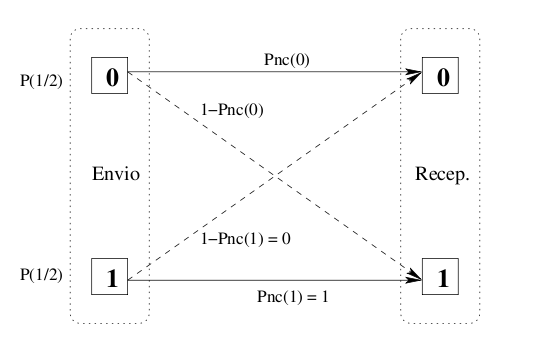
\includegraphics[scale=0.43]{capacidad/canalBinario.png}
  \end{center}
\caption {Canal binario: esquema de probabilidad}
\label{fig:canbin}
\end{figure}

Para calcular el ruido en un canal simétrico binario, calculamos la probabilidad de no-colision que tendra un usuario determinado, ya que las colisiones seran el ruido del canal (En esta etapa no consideramos otros tipos de ruido que pueda tener el canal físico).

\noindent Cantidad de slots por trama: $m$
\noindent Cantidad de usuarios: $n$

\noindent Probabilidad de no colisión para un usuario en un canal simétrico:
\begin{equation}
P_{nc}=\left(\frac{m-1}{m}\right)^{n-1}
\end{equation}


\noindent Probabilidad de no colisión para un usuario en un canal óptico:
\begin{eqnarray}
P_{nc} & = & P(1) \cdot P_{nc}(1) + P(0) \cdot P_{nc}(0) \\
P_{nc} & = & \frac{1}{2} \cdot 1 +  \frac{1}{2} \cdot \sum_{i=0}^{n-1} 
C^{n-1}_{i} \left(\frac{m-1}{m}\right)^i  \left(\frac{1}{m}\right)^{n-1-i}  \left(\frac{1}{2}\right)^{n-1-i} 
\end{eqnarray}

\noindent Donde $\left(\frac{m-1}{m}\right)^i$ es la probabilidad de no
colisión de $i$ canales (se suma para todo posible número de canales no
colisionando: $1\leq i\leq n$, que están en otro slot), $
\left(\frac{1}{m}\right)^{n-1-i}$ es la probilidad de colisión de los restantes
$n-1-i$ (estos están en el mismo slot que el canal actual, el `$-1$' es para no
contar el canal actual), y la colisión se produce cuando los otros canales
transmiten $1$ cuya probabilidad es $\left(\frac{1}{2}\right)^{n-1-i}$. El
factor $C^{n-1}_{i}$ suma sobre todas las combinaciones posibles de canales no
colisionando, que son hechos independientes.

\noindent Teniendo en cuenta que $ \sum_{i=0}^{n-1}
C^{n-1}_{i} \left(\frac{m-1}{m}\right)^i  \left(\frac{1}{2m}\right)^{n-1-i}$ es la potencia $n-1$ de un binomio, reemplanzando tenemos
\begin{eqnarray}
P_{nc} & = & \frac{1}{2} +  \frac{1}{2} \cdot \left(\frac{m-1}{m} + \frac{1}{2m} \right)^{n-1} \\
P_{nc} & = & \frac{1}{2} +  \frac{1}{2} \cdot \left(1- \frac{1}{2m} \right)^{n-1} \\
P_{nc} & \simeq & \frac{1}{2} +  \frac{1}{2} \cdot e^{-1/2} 
\end{eqnarray}

\noindent Donde la última aproximación vale para $n=m$ y $n$ grande.


\vspace{5mm}

\noindent Para el caso de {\em bloom} filters con $k$ filtros\footnote{Se envían $k$ repeticiones del bit en canales distintos, entonces basta que sólo uno de ellos sea 0 para que recibamos un 0 en un canal óptico.} la probabilidad de no colisión es:
\begin{eqnarray} 
P_{nc}^{k} & = &  P(1) \cdot P_{nc}^{k}(1) + P(0) \cdot P_{nc}^{k}(0)\\ \label{Pnc_k}
\end{eqnarray}
Sabiendo que la probabilidad de no colisión para el 0 es:
\begin{eqnarray}
P_{nc}^{k}(0) & = & 1 - \big(P_{c^k}(0)\big)^k 
\end{eqnarray}
Pero la probabilidad de colisión para el 0 cuando se transmiten $k$ copias es:
\begin{eqnarray}
P_{c^k}(0) & = & 1 - \big(P_{nc^k}(0)\big)  \enspace,
\end{eqnarray}
y que además la probabilidad de no colisión para los $k$ slots del bloom
filter es
\begin{eqnarray}
P(\mbox{no col.} k) &=& P(\mbox{no col.}1)\cdot P(\mbox{no col.}2)\cdot P(\mbox{no col.}3)\cdots P(\mbox{no col.}k)\\
&=&\left(\frac{m-1}{m}\right)\cdot\left(\frac{m-2}{m-1}\right)\cdot\left(\frac{m-3}{m-2}\right)\cdots\left(\frac{m-k}{m-(k-1)}\right)\\
&=& \frac{m-k}{m} \enspace.
\end{eqnarray}
Luego la probabilidad de colisión con alguno de las $k$ copias del bit es
\begin{eqnarray}
P(\mbox{col.}k)&=& 1-P(\mbox{no col.} k)\\
&=& 1-\frac{m-k}{m}\\
&=& \frac{k}{m} \enspace.
\end{eqnarray}
Entonces reemplazamos y calculamos:
\begin{eqnarray}
P_{c^k}(0) & = & 1 - \left(\sum_{i=0}^{n-1} C^{n-1}_{i} \left(\frac{m-k}{m}\right)^i \left(\frac{k}{2m}\right)^{n-1-i} \right)  \\
& = &  1-\left( 1-\frac{k}{2m}\right)^{n-1}
\end{eqnarray}
Reemplazando esta ecuación en~\ref{Pnc_k} obtenemos:
\begin{eqnarray}
P_{nc}^k & = & \frac{1}{2} + \frac{1}{2} \left( 1- \left( 1- \left( 1- \frac{k}{2m} \right)^{n-1}  \right)^{k}  \right) 
\end{eqnarray}

Sin embargo, este calculo es incorrecto, comparandolo con los datos que da el simulador. La formula entrega valores de error menores con respecto a los reales, como se observa en la figura. 
Los trazos del mismo color corresponden a el mismo K con azul(K=1), verde (K=2) y rojo(K=4). M=256

\subsubsection{Entropía}

Comenzemos por lo básico:

Segun Shannon, el \textbf{contenido de informacion} h(x) de un suceso x dada la posibilidad que suceda P(x) es:
$$ h(x) = log_{2}\left(\frac{1}{P(x)}\right) $$

Y la entropia de un conjunto A, H(A) se define simplemente como el promedio del contenido de información:

$$ H(A) = \sum_{x E A_{x}} P(x)log_{2}\left(\frac{1}{P(x)}\right)$$

En un canal binario solo dos sucesos existen, uno con probabilidad p, y otro con probabilidad 1-p, por lo tanto para p siendo la probabilidad de error:

$$ H(p) = -p log_{2}(p)-(1-p)log_{2}(1-p) $$

\subsubsection{Entropia condicional}

Vamos a analizar la entropia de dos conjuntos X de entrada y Y de salida interrelacionados.

La entropia condicional de X dado $y=b_k$ donde $b_k$ es un valor dado, es la entropia de la distribucion de probabilidad $P(x|y=b_{k})$:
$$H(X|y=b_{k}) = \sum_{x \in A_{x}} P(x | y=b_{k})\log_2\left(\frac{1}{P(x | y=b_{k})}\right) $$

La entropia codicional de X dado Y es el promedio, sobre y, de la entropia condicional de X dado y:
$$H(X|Y) =  \sum_{xy \in A_{x}A_{y}} P(x,y)\log_2\left(\frac{1}{P(x,y)}\right) $$

\subsubsection{Información mútua}
La información mútua entre X e Y es:
$$I(X;Y) = H(X)-H(X|Y)$$
Mide el promedio de reduccion de la incertidumbre acerca de x que resulta de saber el valor de y, o viceversa: la cantidad promedio de informacion que x revela acerca de y.

\subsubsection{Capacidad de canal}

La capacidad C de un canal discreto sin memoria es :

\begin{equation}
C = \max_{{\cal{P}}_x} I(X;Y) 
\end{equation}

O sea, la máxima información mutua entre los alfabetos X de entrada e Y de salida.
Para hallar el maximo podemos derivar $I(X;Y)$ con respecto a la probabilidad $P_x$.
Para un canal binario asimétrico sin memoria con probabilidad de error $p$, la capacidad máxima $C$ es:

\begin{equation}\label{Cap}
C = 1 - H(p) 
\end{equation}

Si expandimos H(p) en \ref{Cap}:

$$ c = 1-\left(p \times \log_2\left(\frac{1}{p}\right) + (1-p) \cdot \log_2\left(\frac{1}{1-p}\right)\right) $$
Simplificada:
$$ c = 1 + p * \log_2(p) + (1 - p) * \log_2(1-p) $$

Sin embargo esta capacidad es menor que la que realmente tenemos en nuestro canal, ya que un Z-channel se adecua mayormente a los medios de transmisión ópticos. Describiremos en detalle este caso especial en la siguiente sección.

\subsubsection{Canal Z}
Un canal Z (Z-channel) difiere de un canal binario, ya que las probabilidades de bit-flip son asimetricas.
Los Z-channel se usan generalmente para modelar sistemas de transmision opticos.

\begin{figure}[th]
  \begin{center}
    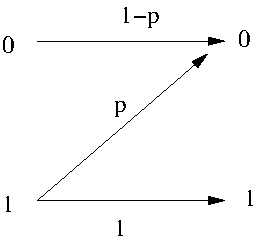
\includegraphics[scale=0.5]{capacidad/zchannel}
  \end{center}
  \caption{Diagrama: Z-channel}
  \label{fig:Gal}
\end{figure}

Para un Z-channel, la distribucion de probabilidades de I(X;Y) es diferente, por lo que obtenemos un máximo diferente:

$$ C_{Z} = 1 - \left(\frac{1}{2}*H(p)\right) $$ \cite{tallini}

Por lo tanto,

$$ C_{Z} = \log_2\left(1+(1-p) p^{p/(1-p)}\right) $$


\begin{figure}[th]
  \begin{center}
    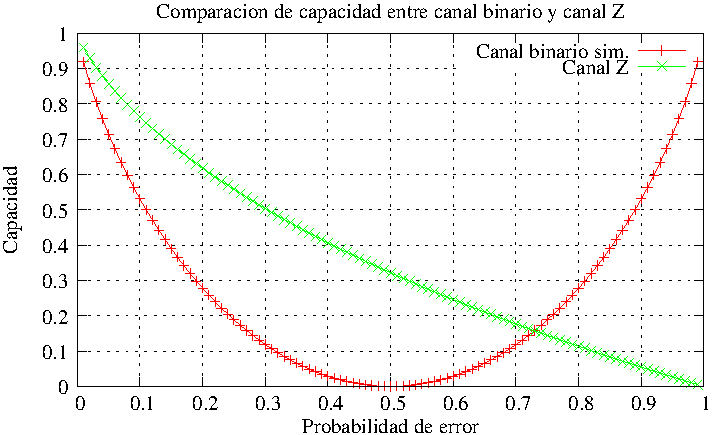
\includegraphics[scale=0.9]{capacidad/comparacionBZ}
  \end{center}
  \caption{Diagrama: Azul: Capacidad de canal binario Verde: Capacidad de canal Z}
  \label{fig:CompBZ}
\end{figure}


\subsubsection{Filtros de bloom}
As discussed in section 2, this leads to collisions. Since the modulation format is OOK, only transmitted ‘1’s can interfere with ‘0’s.
This behaviour can be modelled as a Z-channel because the superposition of individual light pulses representing ‘1’s
can only be identified as a ‘1’, but a received ‘0’ is an unmistakable sign of the absence of pulses in a given time slot.
We found that the Bloom filter [2] provides a convenient structure to correct for errors in this type of channel. This
technique is borrowed from hashing algorithms and is used to test whether an element is member of a given set. The
way that we implement this algorithm relies on copying every bit in K slots of the transmitted frame. On the receiving
end it is sufficient to receive a single ‘0’ out of K copies in order to correctly retrieve the original transmitted ‘0’,
whereas collisions have no effect on ‘1’s.

\subsection{Espectro ensanchado}

Repetido en \ref{espectroensanchado} ??
\subsubsection{Time-hopping con filtros de bloom}

\subsection{Minimización de peso de Hamming}
%% extraido de dline-pub.text
This scheme based on time-hopping CDMA relies on symbol interference for confidentiality as data from other end users effectively acts as noise.
Symbol interference, as discussed in section \ref{principle}, causes errors that need to be corrected.
As these errors reduce the usable channel bandwidth, it is desirable to decrease interference to a point where it still provides security while maximising bandwidth usage.
In order to decrease interference it is not advisable to modify the cryptographically secure random generator, since it would compromise the security of the whole system by introducing predictability in the symbol positions (e.g., using orthogonal codes as in Ref.~\cite{Nadarajah2006}.)
Instead, a strategy based on the fact that an optical channel can be modelled as a Z-channel is pursued.
%This channel presents a Shannon limit of $ C_{Z} = \log_2\left(1+(1-p) p^{p/(1-p)}\right),$ where $p$ is the probability of error~\cite{Tallini:02}.

%Our proposal relies on the characteristic asymmetric nature of this channel type in which only the '1' symbol causes interference.
%In other words, interference is proportional to the Hamming weight of the transmitted symbol.
Hamming-weight of a symbol is the number of bits `1', which is directly related to interferences in the Z-channel.
The Hamming-weight minimisation algorithm consists on coding every binary symbol into an equivalent longer one, having more `0's and less `1's than in the original symbol.
Applying a Hamming-weight minimising algorithm thus decreases interference.
Intuitively, a longer symbol would decrease the channel bandwidth; but as numerical simulations shown (see section \ref{simulations}) as intersymbol interference decreases the FEC overhead can also decrease, compensating for the increase in symbol length and yielding a net bandwidth gain.
Normal binary symbols of length L have variable Hamming weight, with L/2 being the average, zero being the minimum and L being the maximum weight.
We propose decreasing this Hamming weight (HW) to HW=2 a small number, as a good compromise between interference reduction and symbol length.
Additionally, for security purposes we use a fixed Hamming weight for all symbols. This causes a slight loss of bandwidth but makes it impossible to infer any information about the transmitted symbol by analysing statistics of the transmitted data.



\begin{table}[t]
\begin{center}
\begin{tabular}{c c c}
Data & Input HW= 0 to 3 & Expanded HW=2\\
\hline\hline
0 & 000 & 00011\\
1 & 001 & 00110\\
2 & 010 & 00101\\
3 & 011 & 01100\\
4 & 100 & 01010\\
5 & 101 & 01001\\
6 & 110 & 10001\\
7 & 111 & 10010\\
\end{tabular}
\caption{Hamming minimisation table for 3-bit symbols}
\label{hwtable}
\end{center}
 \end{table}
 
\subsection{How the Hamming weight is minimised}
The symbol expansion can be implemented as a lookup table (see table~\ref{hwtable}), where a symbol of length L is used as the index.
The coded symbol has a length N\textgreater L.
For practical implementation purposes it is desirable for L to be either 8 or 16 bits, so the table will have either 256 or 65536 entries.
We apply the Hamming weight minimisation to symbols of 8 or 16 bits of length, thus it is needed a 256 or 65535 output symbols with a HW=2, respectively.
To encode a 16-bits input symbol and HW=2, output symbols of 363 bits long are needed.
% \footnote{For a 8-bit symbol the expanded symbol with HW=2 is 24 bits long}.
Note that the number of unique symbols with HW=2 and N=363 is not exactly 65536 but 65703, so the expansion table is not unique.
The ordering of the symbol conversion is not important as long as the same table is used in all the nodes trying to communicate.
%In general more bits transmitted per frame the more efficient the protocol will be. \textbf{PORQUE IN GENERAL? CUANDO FALLA?} 


\subsection{Sistema completo}
%% De orte.tex
The proposed system is composed of an access layer, where CDMA and error correction are implemented, and a physical layer based on an optical network with certain similarities to PONs. 
The access layer is implemented using time-hopping CDMA, where each of the $128$ possible ONUs sends bits in a slot chosen randomly from a frame of $356$ slots; therefore
collisions between different ONUs will happen and error correction must be used to guarantee error-free data transmission. 
Notice that the synchronization is performed at the bit slot level only because transmission of each ONU is random, in contrast to TDMA where synchronization is also performed at frame level. 
Moreover, each ONU can send data at any time, in contrast to TDMA where
ONUs usually send data continuously; this feature resembles transport by Ethernet frames.
A certain ONU $X$ can receive messages from an ONU $Y$ if $X$ has the
{\em key} of $Y$, and vice versa. Therefore, if a certain group of ONUs
were to communicate over a VLAN, it is required that everyone in the group
knows each others' {\em keys}.
ONUs' data streams are encoded with the following error correction techniques (Fig. \ref{arch:chain}):
 Reed-Solomon ($223/255$) and LDPC ($1024\times512$ matrix) algorithms (see \cite{Moon:05} and references therein), and bloom-filters with $K=4$~\cite{Bloom70space/timetrade-offs}.
The choice of these correction algorithms was heavy influenced by
modeling the optical fiber as a Z-channel, having a Shannon limit of $ C_{Z} = \log_2\left(1+(1-p) p^{p/(1-p)}\right),$ where $p$ is the probability of error. 
This capacity limit is larger than that of a symmetric memoryless binary channel \cite{Tallini:02}.

\subsection{Aplicación en distintos medios físicos}
\subsubsection{Redes ópticas}
% de orte.text
\begin{figure}[!t]
  \centering
    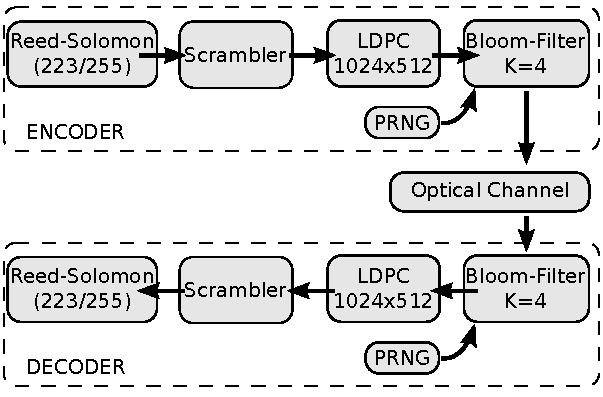
\includegraphics[width=3in]{orte01.pdf}
    \caption{Proposed network design: Access Layer}
    \label{arch:chain}
\end{figure}
% Fiber		Es grave el efecto de la dispersion?  Sugerimos dispersion shifted G.653? O son muy caras?
% splitter	No 1x128 commercially available (attenuation $\leq 27\,dB$)
% DFB		http://cess-dk.com/gfx/upload/PX2-1541SF.pdf ( min $\simeq-1\,dB$)
% APD		http://pdf.dzsc.net.cn/200810212/286762.pdf ( max $\simeq-27\,dB$)
% EDFA		http://www.lambdaphoto.co.uk/pdfs/EDFADatasheet.pdf

The proposed physical layer topology is that of a star (see Fig.
\ref{arch:fig1}) where optical splitters redistribute traffic coming
from each ONU to all the rest allowing point-to-multipoint as well as
point-to-point communications between $128$ ONUs.
%Traffic redistribution is made by optical splitters at the redistribution hub that introduces high attenuation to optical streams.
An Erbium-Doped Fiber Amplifier (EDFA) located in between splitters at
the optical hub increases optical power to overcome network losses.  RZ
modulated optical signals generated at each ONU, of up to $10$~Gbps by a
$2$~dBm $1550$~nm DFB-laser, are transmitted up to $10$~km upstream by a
standard single-mode optical fiber (ITU-T G.652) to the optical hub.

In this hub a $128\times 1$ splitter merges traffic from all ONUs that is then redistributed by a $1\times 128$ splitter channeling back merged traffic to each ONU through a downstream fiber identical and parallel to the upstream fiber.
Splitters' attenuation ($\simeq25$~dB each) contribute, as well as fiber attenuation and insertion losses ($\simeq2$~dB and $\simeq1$~dB per stretch), to high total losses ($\simeq28$~dB at both upstream and downstream paths).
In order to provide signal amplification an EDFA ($\geq27$~dB gain) is placed between both splitters.
This EDFA increases merged traffic power at the first splitter output ($\simeq-26$~dBm `1' active Tx) delivering an adequate power level ($1$~dBm, `1' active Tx) at the second splitter input to provide ONU's receiver a power level for proper reception ($-27$~dBm, `1' active Tx) with a high sensitivity ($-28$~dBm) photodetector (PD).
The PD maximum optical power is not a concern as our simulations show that only up to ten `1' bits collide in any given single bit slot.
Even considering a constant EDFA gain, the PD input optical power would be lower ($-17$~dBm) than that commercial PDs withstand unharmed ($\sim -5$~dBm).
The bit `0' level at PD is given by the addition of the `0' bit transmitted 
by all $128$~ONUs.
The receiver decision threshold should be able to separate between this state and that of a single ONU transmitting a `1' bit.
As the bit `0' transmission power should be very low, imposing
restrictions on the DFB-laser extinction ratio.
The minimal required extinction ratio (`1'$/$`0' peak power ratio) is addressed in the numerical simulations explained next.
% As collisions occur in this scheme minimal powers are such for the case of a single active Tx in a bit slot. In a bit slot with collisions (two or more `1' bits) power increase could be a concern to APD operation
% Optical transmission is performed by a $2$~dBm $1550$ nm DFB-laser generating a
% $10$ Gb/s RZ modulated optical signal, that is transported by up to $10$
% km upstream fiber (ITU-T G.652) to a redistribution hub (see
% Fig.~\ref{arch:fig1}).
\begin{figure}[!t]
  \centering
    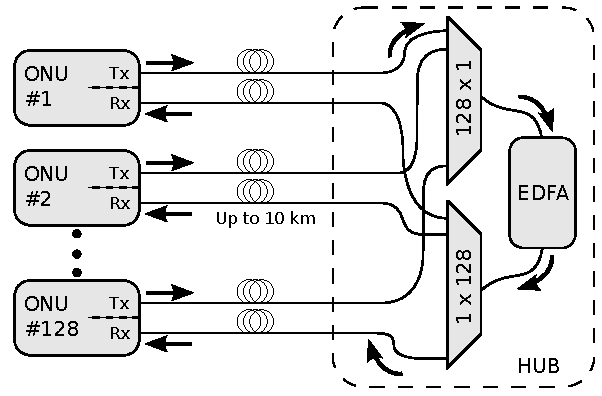
\includegraphics[width=3in]{orte02.pdf}
    \caption{Proposed optical network design: Optical Layer}
    \label{arch:fig1}
\end{figure}
% Upstream traffic from all ONUs are merged by a $128\times 1$ splitter and then again redistributed by another splitter $1\times 128$ that channels back merged traffic to each ONU through a downstream fiber identical and parallel to the upstream one.
% Splitters' attenuation ($\simeq25$~dB, estimated) contribute, as well as fiber attenuation and insertion losses ($\simeq2$~dB and $\simeq1$~dB per stretch), amount to high total attenuation ($\simeq28$~dB at each upstream and downstream paths).
% In order to make the system workable it is proposed to place a single EDFA optical amplifier ($\geq27$~dB gain) between both splitters.
% This EDFA rises merged traffic power at first splitter output ($\simeq-26$~dBm `1' active Tx) delivering enough power ($1$~dBm, `1' active Tx) at second splitter input to assure power reaching each ONU ($-27$~dBm, `1' active Tx) allows proper reception by a high sensitivity APD ($-28$~dBm).

\subsubsection{Redes acústicas}
% de newJIS_140512-1.pdf (paper JIS)
\begin{figure}[!t]
  \centering
    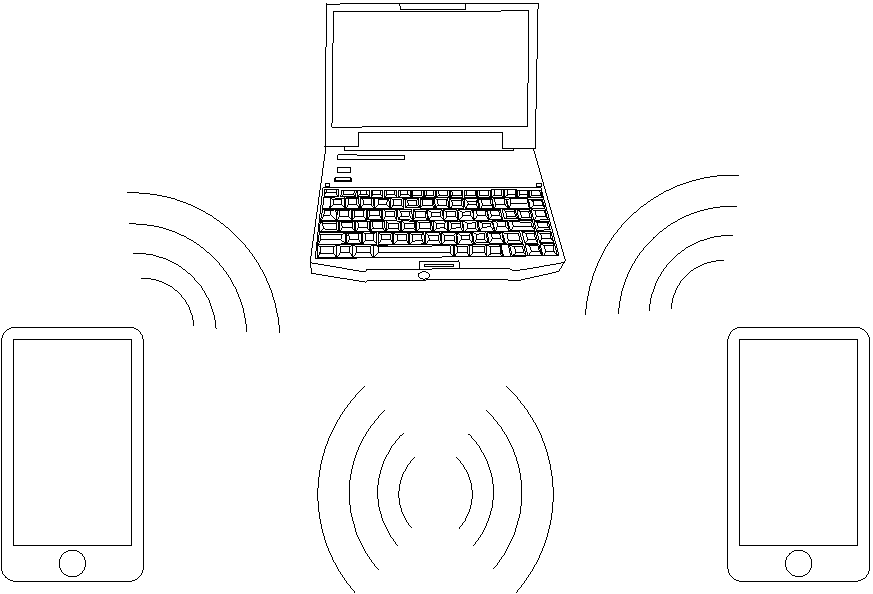
\includegraphics[width=3in]{compucelus.pdf}
    \caption{Proposed acoustic network may have heterogeneous nodes like cell-phones and personal computers.}
    \label{arch:chain}
\end{figure}


Optical links present as their main drawback the requirement of a clear line of sight between devices, a condition which cannot be guaranteed in some working environments. Moreover, they require the installation of additional light sensing hardware on devices not equipped with cameras, or even infra-red transceivers.
Acoustical communications, however, can operate using standard hardware microphones and speakers, ubiquitous on information devices [6]. Furthermore, line of sight is not required to establish links among nodes which can be placed up to a meter apart, emitting low volume audio.
Unlike other technologies, e.g., optical fiber communications, the broadcast nature of sound waves makes privacy safeguards an essential requirement. Several audio communication systems have been proposed [7], but to the best of our knowledge, the question of privacy has been addressed only in the application layer using security protocols. We present a physical layer approach to secure acoustical communications based on time-hopping CDMA, similar to those presented in references [8, 9]. In this work we present a point-to-point or point-to-multipoint secure acoustic network which has a short range and consumes a negligible amount of power, requiring no additional hardware on mobile clients.
Establishing a private link among previously un-paired mobile devices based on software privacy schemes requires some degree of user interaction that is usually neglected [5]. However, when privacy is dealt at the physical layer user intervention is minimized; that is the case in our proposal.
An envisioned application scenario for this technology is the validation of small financial transactions such as PoS (Point of Sale) or ATMs using an unmodified mobile device (e.g. a smartphone). A similar technology addressing these user cases is Near Field Communications (NFC) [10], a wireless protocol which requires specialized hardware not currently present in most mobile devices.

\subsubsection{Redes acusticas: Arquitectura}
The main advantage of the proposed system is the simplicity, just a sound emitter (speaker), a receiver (microphone) and a sound media channel are needed; and those are already available in computers, tablets and cell-phones. It is composed by Secure Time-hopping CDMA running over the sound media channel, error corrections algorithms, and a synchronization method. As a result, the system provides unidirectional users’ channels for point-to-point and multicast communications, while bi-directional communications can be established using two separate channels (i.e., two different CDMA codes in the same media), or by employing the same channel in half-duplex. The later proposition needs further developing work and falls beyond the scope of this paper.
We provide further details in the following subsections.


\section{Experiencias realizadas (mediciones)}
\subsection{Implementación en software}
\subsubsection{Reed-Solomon}
\subsubsection{Bloom-filter}
\subsubsection{Simulador de ruido óptico}
%% de orte.text
The physical optical channel simulation block provides an estimate of
the BER performance of the optical channel. Simulation steps are as
follows: RZ upstream traffic coming from all ONUs is assumed to arrive
at the $128\times1$ splitter with perfect time synchronization, i.e., there is no timing jitter. 
%This allows to simulate merged traffic as a simple addition of optical intensities at bit slots for either `0' or `1' bits. % borrar!
The `0'-bit slots contain a small CW optical intensity given by the Tx extinction ratio. 
Each on-line ONU adds its `0'-bit optical intensity yielding a base power level.
% As many bit `0' optical intensities are added as on-line ONUs to produce a base power level.  
Each `1'-bit adds a super-Gaussian ($m=4$) pulse, duty cycle $1/3$, to the base power level. %, with rising edge at slot start and peak amplitude accordingly to Tx optical mean output power.
% As many bit `1' intensities are added to base level as active Tx there are at each simulation bit slot.
 
Upstream and downstream merged traffic suffers from attenuation due to
splitter, fiber, and
splice losses. The power budget is balanced by an EDFA with $27$~dB constant gain.
Amplified spontaneous emission from the EDFA is modeled by white Gaussian
noise, with intensity proportional to the amplifier noise figure ($7$~dB), and is added
after the EDFA. 

%Real EDFAs gain increases with higher input power, i.e. amplification is not
%linear with number of active Txs. Settling for worst case scenario simulation
%we assume same $27\,dB$ gain for any number of active Txs. ASE noise produced
%at EDFA is modelled as a white Gaussian noise added to the optical signal. An
%EDFA accomplishing the amplification previously discussed ($-25.5\,dBm$ to
%$1.5\,dBm$) would have an output SNR $\geq 60\,dB$ accordingly to a estimation
%based on the bandwidth of forthcoming optical filtering at APD detector (see
%section 6.5.1 at~\cite{Agrawal:xx}). Dispersion compensation regeneration stage
%operation is accounted for by simulating no dispersion effects. Traffic is
%routed back to all ONUs by a 1x128 splitter through another $10\,km$
%fiber,
%amounting to a $27.5\,dB$ attenuation; so for one active Tx input power at each
%Rx would be $-27\,dBm$.

The input optical signal at the receiver is filtered (2nd order low-pass Butterworth filter, $25$~GHz bandwidth) and photodetected assuming a standard PD responsivity (see section 4.4.3 of~\cite{Agrawal:xx}).
White Gaussian noise accounting for thermal and shot noise is then added
to the photocurrent, and 
electrical filtering is applied (2nd order low-pass Butterworth filter, $14$~GHz bandwidth).
%Simulating the decision process a mean of samples around maximum eye opening is compared to a threshold current. 
%Current in case of `1' bits collision is higher than that of a single active Tx, so threshold is established assuming that later case.

%Real EDFAs gain increases with higher input power, i.e., amplification would not be linear with number of active Txs. 
%Settling for worst case scenario simulation we assume same $27\,dB$ gain for any number of active Txs. 
%ASE noise produced at EDFA is modeled as a white Gaussian noise that's added to the electric field. 
%An EDFA accomplishing the amplification previously discussed ($-25.5\,dBm$ to  $1.5\,dBm$) would have an output SNR $\geq 100\,dB$ accordingly to a estimation based on the bandwidth of forthcoming optical filtering at detector (see section 6.5.1 at~\cite{Agrawal:xx}). 
%Effect on traffic of dispersion compensation regeneration stage is accounted by not including in the simulation pulses deformation due to dispersion. 
%Afterwards traffic is routed back to all ONUs by a $1\times128$
%splitter through another $10\,km$ fiber, amounting to a $27.5\,dB$ attenuation arriving to each Rx with $-27\,dB$ for one active Tx.
%
%A concern was if maximum mean total input power allowed at Rx would be surpassed when multiple Tx were simultaneously active. 
%Simulation shown that the occurrence of 15 simultaneously active Tx was a very rare event {\bf <CUANTO??>}. 
%That would amount to $\sim-15\,dBm$ reaching each ONU Rx, well bellow standard commercial Rx overload of $\sim+0.5\,dBm$, that's maximum acceptable mean input power for a BER$<1\,10^{-12}$. 
%
%Rx optical bandwidth is simulated as a low pass filter (2nd order Butterworth as a digital IIR filter~\cite{IIR}, cutoff frequency $25\,GHz$). Afterwards optical traffic is converted into an electrical current. Then to account for thermal and shot noise at a typical APD white Gaussian noise current is added, with an estimated SNR $\simeq 42\,dB$ (see section 4.4.3 at~\cite{Agrawal:xx}). Then electrical filtering is applied (2nd order Butterworth IIR filter, cutoff frequency $6\,GHz$). Detection procedure is performed by comparison to a fixed current threshold. A previous simulation run with the same number of ONUs but with a single active Tx allows to determine the decision threshold at the time of maximum eye diagram opening. Addition of bit `1' amplitudes (collision) produce a current even higher than for a single active Tx, thus this bit slot will be classified as `1' at optical channel simulation output. 
%Media block account for fiber, EDFA and splitters. It attenuates optical trains (splitters and fiber attenuation minus EDFA gain) and also adds white Gaussian noise to the electric field accounting for ASE noise at EDFA. 
% MUCHO, MUY IMPORTANTE: REVISAR CALCULO OSNR (Fn) y verificar que se determina en detector %[VAB]
% ITU recommendation G. 959.1 states that certain interfaces' should operate normally up to $12\,dBm$ mean total input power. In any case if such power is surpassed it would only cause a very short time blinding of Rx affecting a so small amount of bits that wouldn't affect the logical layer ability to correct them.
% receiver overload: max input power for BER<1E-12
%Receiver block simulates Rx behavior. It's optical bandwidth is taken into account by simulating a low pass filtering of incoming traffic (2nd order Butterworth as a digital IIR filter~\cite{IIR}, cutoff frequency $25\,GHz$). Then optical traffic is converted into an electrical current. White Gaussian noise current is added to account for thermal noise at Rx, being it's SNR $\simeq 42\,dB$ accounting for thermal and shot noise at a typical APD detector (see section 4.4.3 at~\cite{Agrawal:xx}). Afterwards another filter simulates detector's linear channel (2nd order Butterworth IIR filter, cutoff frequency $6\,GHz$). Detection procedure is performed by comparison to a fixed current threshold. A previous simulation run with same number of ONUs but with a single active Tx allows to determine the decision threshold at the time of maximum eye diagram opening. Addition of bit `1' amplitudes (collision) produce a current even higher than for a single active Tx, thus this bit slot will be classified as `1' at 
optical channel simulation output. 


%\section{Simulation results}
Noise fluctuations at power levels near the PD sensitivity limit have an important effect on signal detection. 
%Detection being made at power levels near PD sensitivity is highly sensitive to changes in noise.
Shot noise is of particular concern as it is proportional to the mean photocurrent.
In our network proposal the later is higher than in PONs as bit
`0' optical intensities from all ONUs are added.
The resulting base-level optical intensity is then heavily dependent on the Tx extinction ratio.
Fig.~\ref{sim:optical} shows minimal extinction ratios required to
achieve an arbitrary BER in the physical layer as a function of the
number of on-line ONUs.
\begin{figure}[!t]
    \centering
      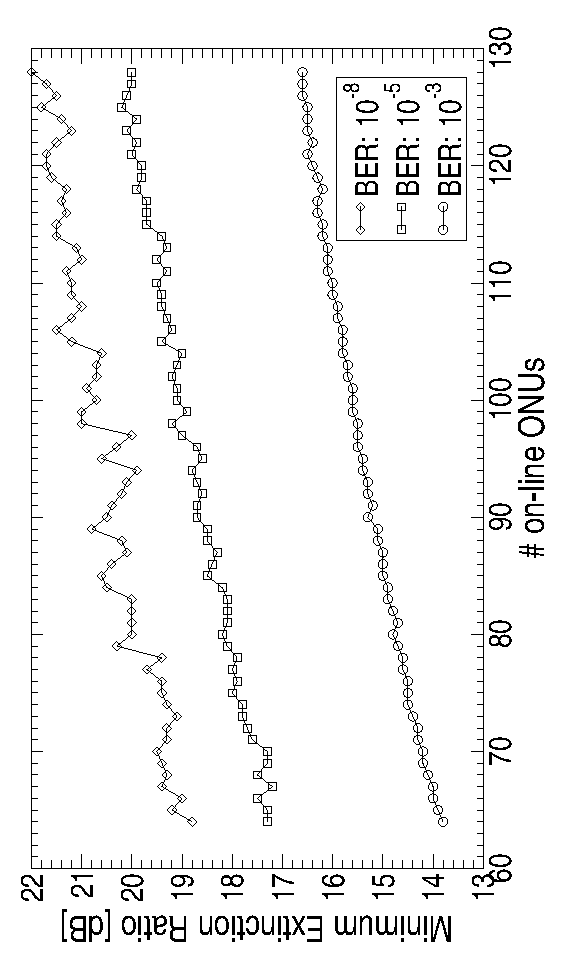
\includegraphics[angle= 270, width=3.5 in]{orte03.pdf}
      \caption{Physical layer simulation result: Minimal extinction ratio required to assure a given BER}
      \label{sim:optical}
\end{figure}
In the $128$ ONUs scenario a  BER$<10^{-3}$ can be achieved using
commercially available transmitters with an extinction ratio $\simeq16.6$~dB.
This BER is low enough to allow for logical-channel error-correction routines that guarantee error-free transmission, while still making use of a fair fraction of channel capacity.
% perform correctly and still use a fair fraction of channel capacity.
% Fig.~\ref{sim:optical} shows simulation results for the BER vs OSNR
% for different numbers of ONUs with fixed electrical SNR $\simeq 42$~dB.
% Higher BERs as ONUs number increases due to the higher probability of
% simultaneous bit `1' transmissions (collisions) yielding pulses of
% optical power higher than that of a logical
% `1', generating intersymbol interference. Higher powers generate higher
% currents at Rxs that demand longer times to settle to logical `0' levels after
% filtering. Nevertheless, as
% can be seen in fig.~\ref{sim:optical}, in the worst case scenario (128
% ONUs) the expected OSNR at the EDFA output is enough ($\geq 40$~dB) to
% ensure a BER$<10^{-7}$. In this case simulation shown that the occurrence of
% 15 simultaneously active Tx was a very rare event, so optical power at Rx
% would be $\simeq -15$~dBm, well bellow standard commercial Rx overload
% of $\sim0.5$~dBm (maximum acceptable mean input power for a
% BER$<10^{-12}$).
\begin{figure}[!t]
    \centering
      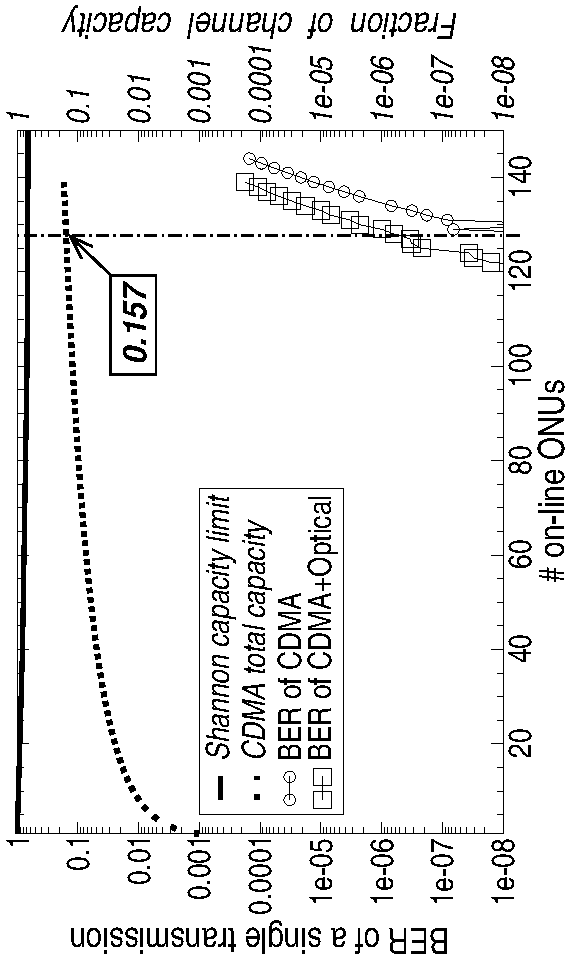
\includegraphics[angle=270 ,width=3.5 in]{orte04.pdf}
    \caption{Simulation results: Logical channel}
      \label{sim:access}
\end{figure}
Fig.~\ref{sim:access} shows simulation results for the fraction of the total
capacity and the BER of one channel at the coding level (circles) and 
including physical layer impairments (squares). These results were obtained by
sending one Gigabit of data for each ONU simultaneously.
This figure shows a channel utilization of $15.7\%$ when all of $128$ ONUs
are transmitting simultaneously, with a BER$<10^{-8}$. 
From Fig. \ref{arch:fig1} we observe a penalty of $8$ ONUs when
impairments from the optical layer (mainly extinction ratio and noise from EDFA and PDs) are taken into account.
Considering that the system was designed to support asynchronous communications (e.g., Ethernet), it is not likely that all the ONUs will transmit simultaneously (e.g., Internet links often operate at most at $90\%$ load); and therefore our system has a BER $<10^{-8}$ for each channel when 119 ONUs are transmitting at a same time ($119/128>0.9$).
%, removing only one ONU re-establish the desired BER. 
%
%It is worth to remark that, even if the optical channel can induce a
%significant number of errors, the access layer has shown to be able to correct a
%very large number of errors (it is based on
%LDPC+Reed-Solomon+Bloom-Filters), as can be seen on the curve with squares
%at fig.~\ref{sim:access}.
Observe that the high error rates correspond to a
worst-case scenario when all ONUs are transmitting simultaneously at
full capacity, and also 
there is a low penalty due to physical layer impairments.
%Figure~\ref{sim:optical} presents the simulation's BER vs optical OSNR
%for different numbers of ONUs. %[VAB]
%As the number of ONUs increases higher BERs are obtained at the same optical SNR (electrical SNR is fixed at $\simeq 42\,dB$). In particular there is a penalty of about $30\;dB$ for 128 ONUs in comparison to 1 ONU. This is expected as a consequence of the higher probability of simultaneous bit `1' transmissions (collisions) yielding pulses (logical `1's) of different powers (sum of the power of each transmitter). Higher powers demand more time to settle post filtering current to logical `0' levels. If the following bit slot is indeed a logical `0' an erroneous determination is more possible with a higher collision probability. Nevertheless it can be inferred from simulation results that optical channel should not add significantly to the BER for the whole link as the estimated optical SNR of $\geq 100\,dB$ even for the worst case scenario with 128 ONUs present.
% \begin{figure}[!t]
%     \center
% %     \subfigure[Optical channel]{
% %      \label{sim:optical}
%       \includegraphics[scale=0.4]{BERvsSNR_6GHz.pdf}
% %    }
% %    \subfigure[Logical channel]{
% %      \label{sim:access}
%       \includegraphics[scale=0.4]{BERvsONUs.pdf}
% %    }
%     \caption{Simulation results}
%       \label{archfig}
% \end{figure}

\subsection{Implementación en FPGA}
El estudio de PONs plantea el desafío de generar, transmitir y recibir
señales de 10 Gbps en el laboratorio. El costo de estos sistemas
suele ser muy elevado. En este trabajo proponemos una alternativa de muy
bajo costo basada en la generación y trasmisión de señales en FPGAs.

\subsubsection{Arquitectura alto-nivel de la FPGA Xilinx ML507}
El equipamiento consta de un kit de desarrollo ML-507 de Xilinx y un
transceptor SFP+ con láser de 1330 nm, con capacidad de hasta 10 Gbps
en modulación NRZ y alcance de 10km en fibra monomodo. Para realizar
las mediciones presentadas en este trabajo se utilizaron dos dispositivos:
\begin{itemize}
 \item {\em Integrated Bit Error Rate Tester} (iBERT) \cite{4gtxs}: Es
un medidor de tasa de error que utiliza un analizador lógico embebido dentro
del mismo diseño de la FPGA, con interfaz para la herramienta de
verificación y depuración ChipScope. Mediante este agregado, que debe
ser sintetizado dentro del diseño, es posible medir en tiempo real
varios parámetros del transceptor asi como realizar estadísticas y
mediciones de error, variando tasas y características de la transmisión
en tiempo real.
 \item Osciloscopio Óptico Agilent 86100A con módulo óptico 86105A: Para
realizar las mediciones físicas contamos con este equipo que posee un
ancho de banda de 20 Ghz en potencia óptica, suficiente para capturar en
tiempo real los bits individuales o realizar un diagrama de ojo.
\end{itemize}
\subsubsection{Transmisión a multi-gigabit}
\subsubsection{Diseño del sistema propuesto}
\subsection{Redes ópticas}
% de confEUA.tex

\subsubsection{Transmisión a 9 Gbps con SFP+}
El montaje para la experiencia se realizó conectando el transceptor SFP+
al conector correspondiente en la placa de desarrollo ML-507 y un bucle de
fibra óptica ({\em loopback}), con el objetivo de realizar las
mediciones de BER. Luego, para realizar las mediciones con el
osciloscopio, se debe conectar el extremo de recepción de la fibra
óptica al osciloscopio. En este caso generamos el disparo del
osciloscopio mediante la señal de reloj del sistema (placa ML-507) que
se obtiene a través de los conectores SMA J12 y J13 (si bien es
diferencial sólo utilizamos uno de ellos).  Para la depuración y
configuración se utilizó la interfaz JTAG USB de Xilinx ``Platform Cable
USB II''.
\subsubsection{Configuración del reloj del transceptor}

La tasa de transmisión del transceptor GTX está dada por la
frecuencia de reloj de entrada $F_{PLL\_Clock}$, donde se transmite un
bit por cada semiciclo (la modulación es NRZ); entonces la tasa de
transmisión será
$R_{line}\mbox{[bps]}=F_{PLL\_Clock}\mbox{[1/s]} \times 2$.  La
frecuencia del reloj de entrada del PLL está gobernada por la ecuación
5-1 \cite[Pag. 88]{ug198}, que reproducimos a continuación:

\begin{equation}
F_{PLL\_Clock} = F_{CLKIN} \times \frac{PLL\_DIVSEL\_FB \times
DIV}{PLL\_DIVSEL\_REF}% \enspace
\end{equation}\\

donde las constantes $PLL\_DIVSEL\_REF = \{1;2\}$, $DIV = \{4;5\} $ y
$PLL\_DIVSEL\_FB = \{1;2;3;4;5\}$ son configurables por software;
mientras que la frecuencia base se configura con las llaves
SW6~\cite[Tabla 1-32]{ug347}: $
F_{CLKIN} (Mhz)= \{62.5;75;77.76;100;125;150;156.25;311.04;622.08\}$.


 Modificando los parámetros puede lograrse, en teoría, un amplio rango
de la frecuencias $F_{PLL\_Clock}$, pero de acuerdo a la documentación
del PLL \cite[Pág. 71]{ug366}~\footnote{La velocidad máxima no se
detalla en la documentación del GTX de Virtex5, pero si en la
documentación del Virtex6, que excepto en el modelo HTX posee parámetros
similares.}, este tiene un rango de operación nominal desde $1.2$ a
$2.7$ Ghz en FPGAs de grado $-1$ tal como el que se encuentra en la
placa de desarrollo ML-507. Sin embargo en este artículo documentamos la
obtención y medición de velocidades de oscilación estables para el PLL
de hasta $4.5$ Ghz (lo que implica una tasa de transmisión de $9$ Gbps),
fuera del rango de operación especificado por el fabricante.

\begin{figure}[t]
  \centering
    %\includegraphics[scale=0.70]{plot.png}
    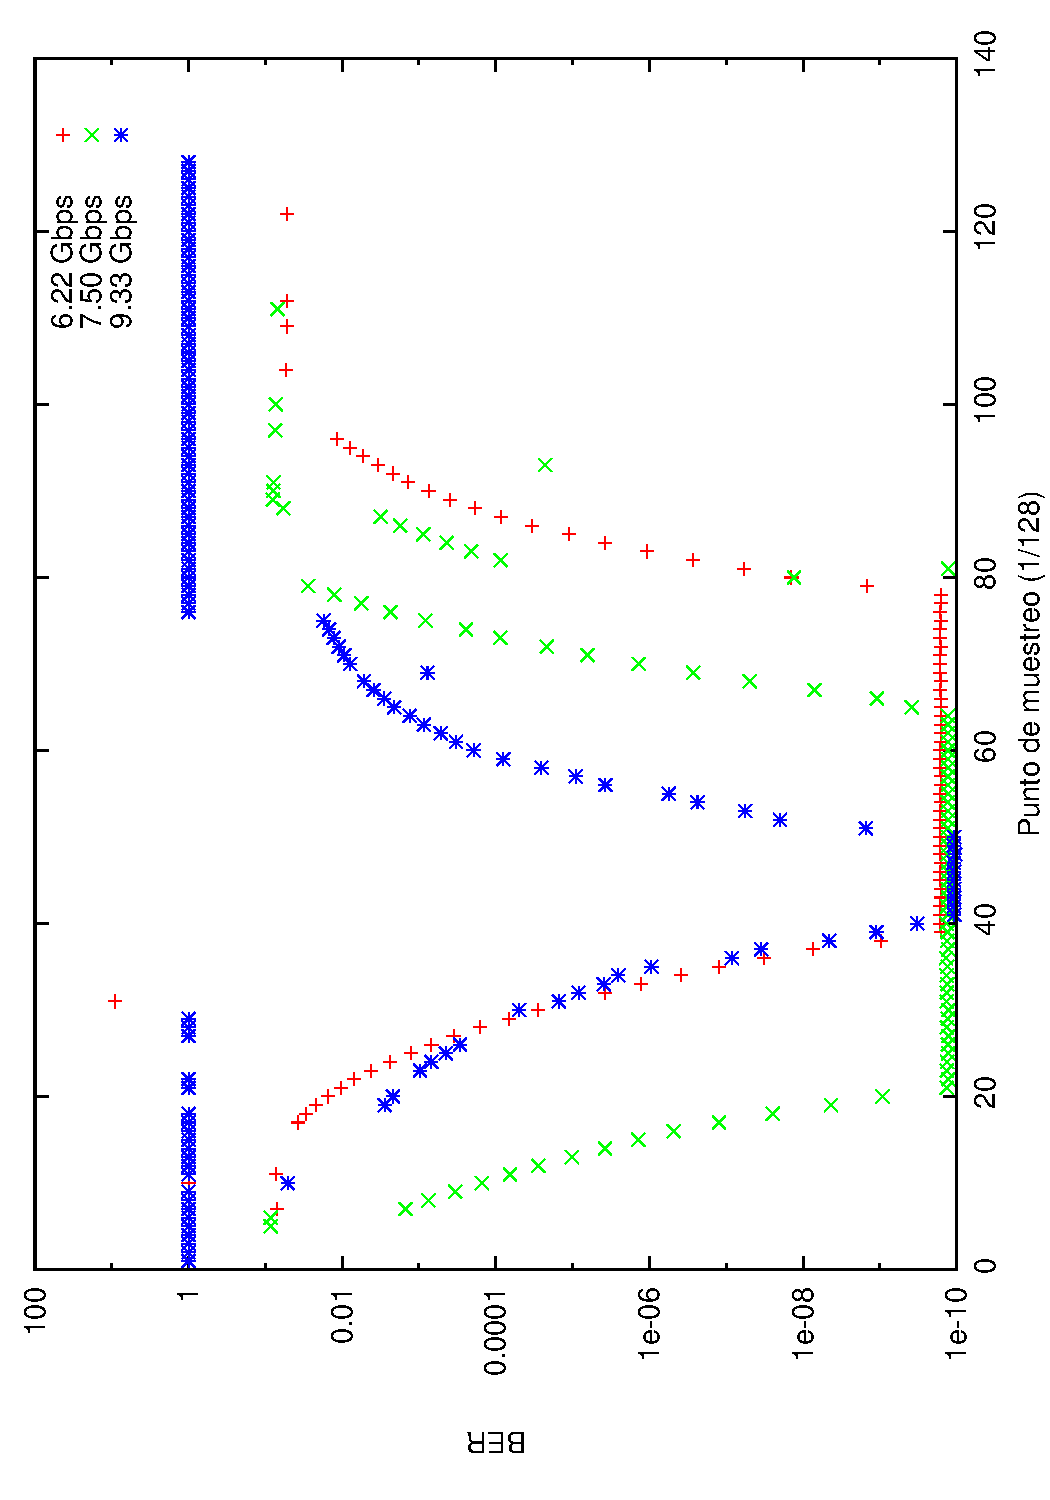
\includegraphics[width=6cm,angle=270]{medicionesPaper/BER_sp.pdf}
\caption {BER vs. punto de muestreo.}
\label{fig:BER}
\end{figure}
\section{Mediciones}
\begin{figure}[!t]
  \centering
%  \subfigure[$4.5$ Gbps]{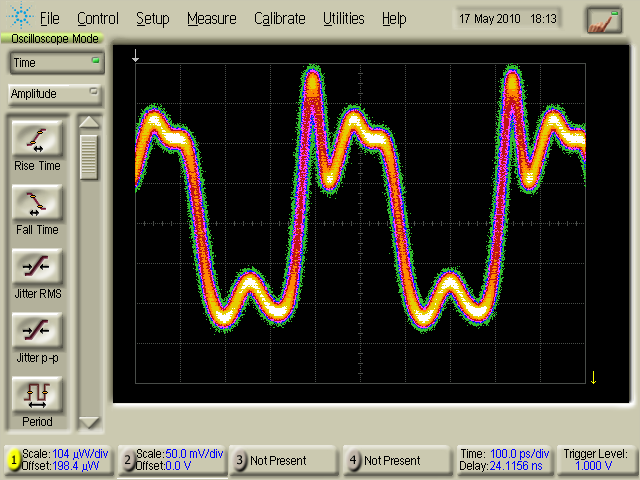
\includegraphics[scale=0.52]{medicionesPaper/screen3.png}
  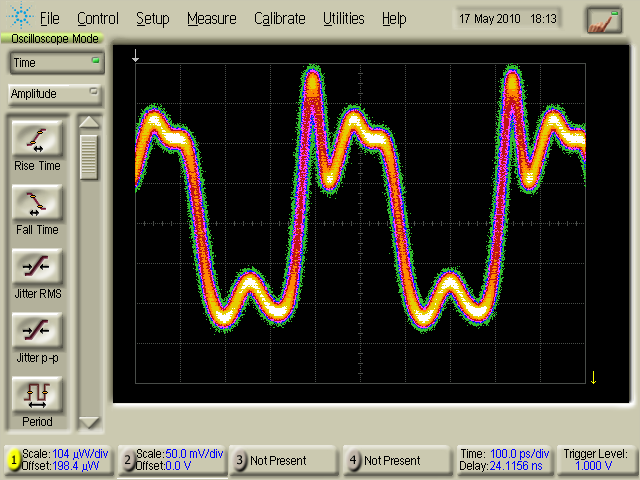
\includegraphics[scale=0.52]{medicionesPaper/screen3.png}
  \caption {Señal óptica a $4.5$ Gbps}
  \label{fig:Img1}
%  \\[1cm]
\end{figure}

\begin{figure}[!t]
  \centering
%  \subfigure[$6$ Gbps]{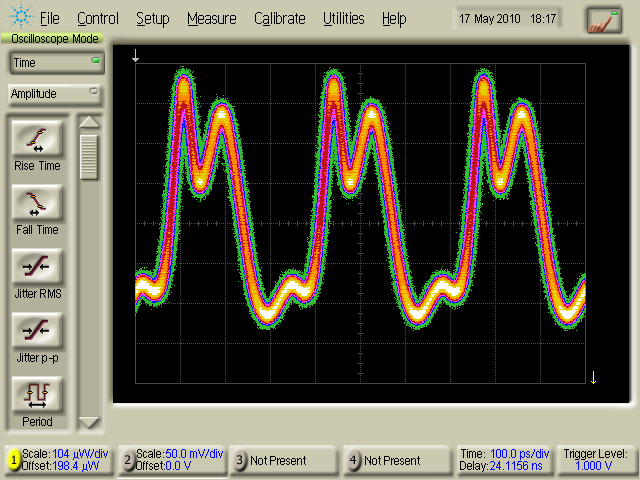
\includegraphics[scale=0.52]{medicionesPaper/screen4.png}
 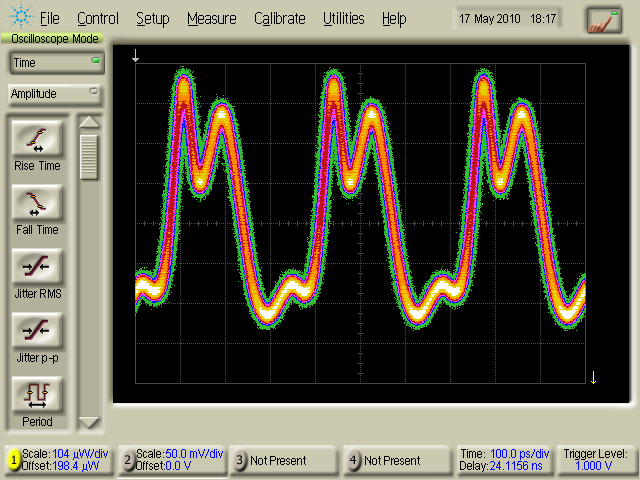
\includegraphics[scale=0.52]{medicionesPaper/screen4.png}
  \caption {Señal óptica a $6$ Gbps}
  \label{fig:Img2}
%  \\[1cm]
\end{figure}

\begin{figure}[!t]
  \centering
%  \subfigure[$7.5$ Gbps]{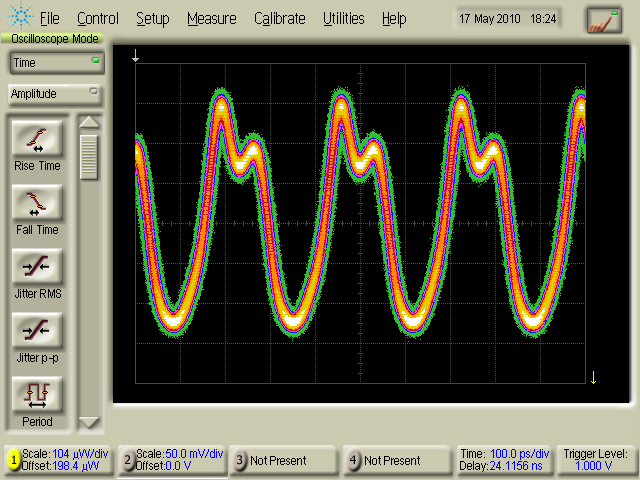
\includegraphics[scale=0.52]{medicionesPaper/screen5.png}
 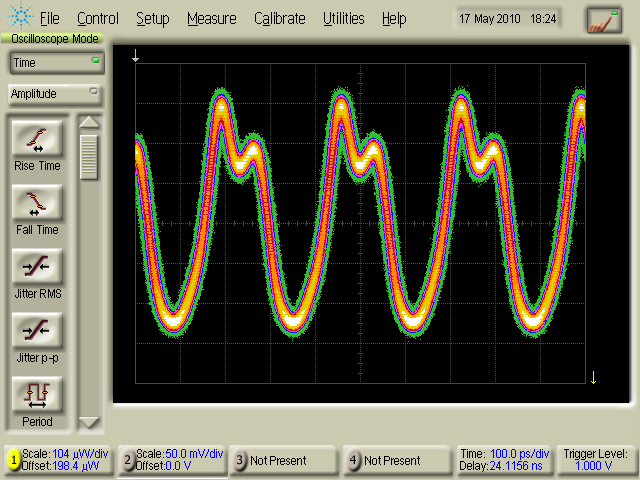
\includegraphics[scale=0.52]{medicionesPaper/screen5.png}
  \caption {Señal óptica a $7.5$ Gbps}
  \label{fig:Img3}
%  }
\end{figure}


\begin{figure}[!t]
  \centering
%  \subfigure[$9.33$ Gbps]{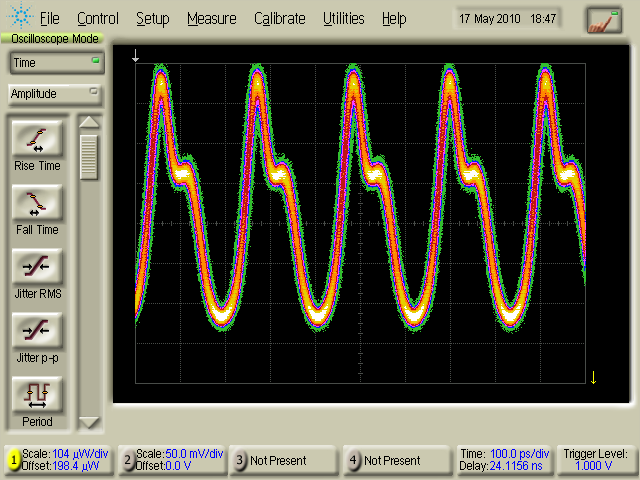
\includegraphics[scale=0.52]{medicionesPaper/screen6.png}
 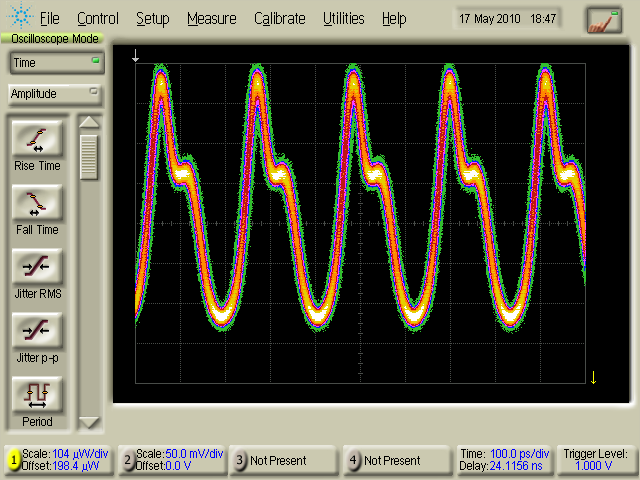
\includegraphics[scale=0.52]{medicionesPaper/screen6.png}
  \caption {Señal óptica a $9.33$ Gbps}
  \label{fig:Img4}
%  }\\[1cm]
\end{figure}


\begin{figure}[!t]
  \centering
%  \subfigure[$12.44$ Gbps]{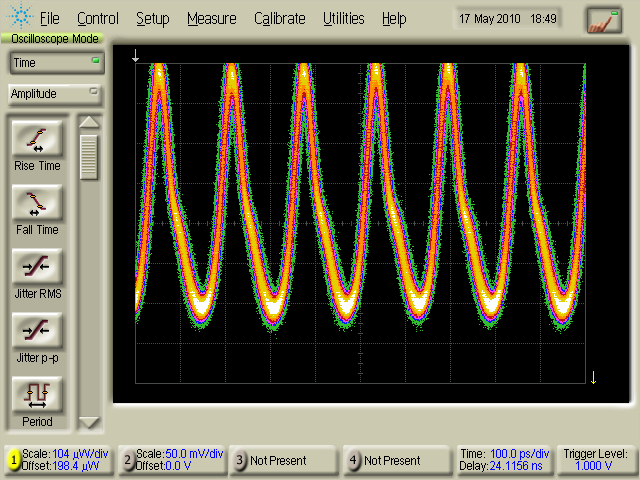
\includegraphics[scale=0.52]{medicionesPaper/screen7.png}
 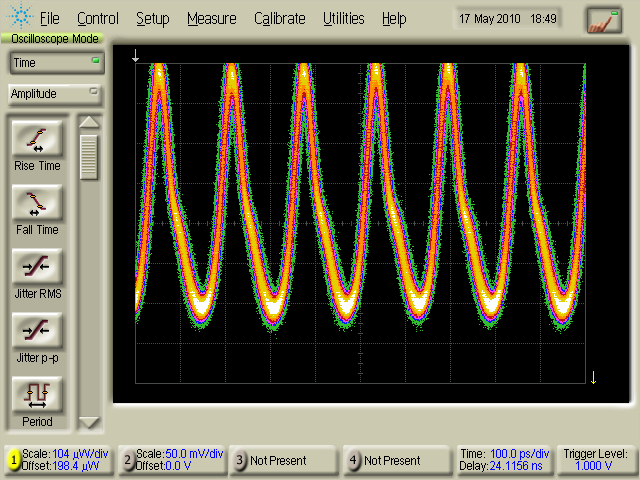
\includegraphics[scale=0.52]{medicionesPaper/screen7.png}
  \caption {Señal óptica a $12.44$ Gbps}
  \label{fig:Img5}
%  }
\end{figure}



\begin{figure}[!t]
  \centering
  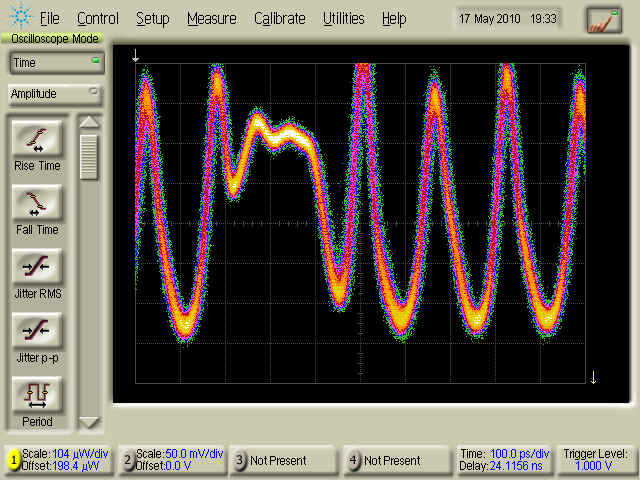
\includegraphics[scale=0.52]{medicionesPaper/screen12.png}
  \caption {Señal óptica a $12.44$ Gbps, transmisión 10110101010}
  \label{fig:Img6}
\end{figure}



Las figuras \ref{fig:Img1} a \ref{fig:Img5} muestran la señal óptica producida a diferentes
tasas. Nótese que aunque el equipo puede generar señales estables de
hasta $12.44$ Gbps pero no puede recibirlas a esa frecuencia, por lo que las
mediciones de BER se realizaron solo hasta $9.33$ Gbps. Todas las señales
corresponden a la secuencia 10101010, excepto la figura \ref{fig:Img6},
que fue generada con una secuencia distinta para demostrar el total
control sobre la señal generada. El transceptor posee la capacidad de
realizar una codificación 8B/10B adicional, pero para estas mediciones
ese módulo fue desactivado.



\subsubsection{Implementación del sistema sobre 8B/10B}
\subsection{Redes acústicas}
\subsubsection{Sincronización}
% de newJIS_140512
On-Off Keying modulation of sound waves, following the Z-channel interface model described in Section 2.2., encode the transmitted bits as pulses. Carrier frequency can vary from 10 kHz to 16 kHz. Good results can be obtained with a rate of 1000 bps at frame level. In experiments, delay (the time for a bit to traverse the network) was very high, due to Reed-Solomon 223/255 coding, a frame to support up to 16 users and the low capacity of the physical media. A more sensible choice of FEC algorithm (like BCH [12]) could drastically reduce data delay. Simple pulse shaping is realized using a pass-band filter at the output of the modulation and also at the input of the demodulator. This filter also helps reject unwanted interference.
As it follows from the description of the communication channel, synchronization between the transmitter and receiver is essential for the correct decoding of information. For this purpose, an initial synchronization pattern is sent, so the receiver can adjust parameters like phase and decision level (see Figure 3). For the data bits transmission a duty cycle of 50\% showed in our experiments an enhanced detection. Clock drift and jitter are not significant at this low transmission speed and so no correction is required, making the software modem implementation very simple. Decision level is dynamic, meaning it is constantly re-calculated from averaged input data. The receiver symbol phase is also corrected using the input data as reference. Notice that this simple synchronization method allows detecting the frame start as well as the bit slot; both are needed at every communication. Moreover, once the data began to be transmitted, the communication becomes indecipherable thanks to the CS-PRNG.

\subsubsection{Modulación}
\subsubsection{Medición multi-usuario}
\subsubsection{Medición distintas distancias}

\section{Conclusiones}

%\bibliographystyle{plain}
\bibliographystyle{IEEEtran}
\bibliography{vb_fgct,IEEEabrv,IEEEorte,confEUA}

\end{document}
